\begin{center}
\textsc{\Large Laboratorio 8}~\\
{\large Vídeo Juegos, Programación, Diseño}~\\
\emph{Menús e Interfaz de Juego}
\end{center}

\section{Pre-Laboratorio}
\todo[inline]{Por hacer.}

\section{Introducción}
\setlength\intextsep{0pt}
\begin{wrapfigure}[9]{l}{0.4\linewidth}
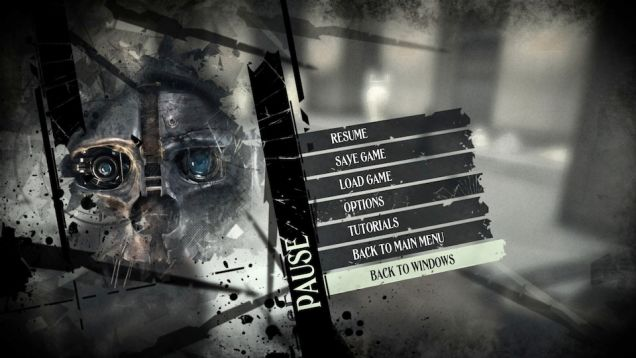
\includegraphics[width=\linewidth]{semana8/dishonored_menu.jpg} 
\caption{Menu de Inicio del juego \emph{Disnohored} \cite{dishonored}.}
\end{wrapfigure}
Los vídeo juegos durante su ejecución presentan variados sistemas de interfaces, menús y pantallas de información al usuario, en la mayoría de los casos los juegos presentan como mínimo una pantalla de inicio con la opción de empezar el juego y salir de el mismo, otro menús muy común es el menú de opciones en el cual se presentan una variedad de personificaciones sobre ciertos parámetros del juego \cite{gb_optionsmenu}. Es usual que en plataformas como el computador personal se presenten mayor numero de opciones en el menú de opciones tales como opciones gráficas y de performance debido a la variada cantidad de configuraciones de hardware, en otras plataformas como las consolas es común que solo se presenten modificaciones sobre el audio del juego, dificultad o re-configuración de los controles de juego.
\newpage
\section{Menús e Interfaces Comunes}
\setlength\intextsep{0pt}
\begin{wrapfigure}[8]{r}{0.3\linewidth}
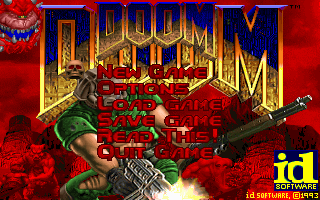
\includegraphics[width=\linewidth]{semana8/doom_start.png} 
\caption{Menu de Inicio del juego \emph{DOOM II} presenta inicio de juego, opciones, guardar y cargar partidas y salida del juego \cite{doomii}.}
\end{wrapfigure}
Las necesidades de interfaces, pantallas y menús cambian según los requerimientos de diseño de cada juego, sin embargo se presentan acá los componentes de interfaz y menús encontradas en la mayoría de los vídeo juegos actuales.
\subsection{Menú de Inicio o Menú Principal (Start Menu o Main Menu)}
Es la primera interfaz que encuentra el usuario al iniciar el juego, presenta por lo menos la opcion de iniciar el juego y salir del mismo, tambien se suelen incluir opciones como ir al \emph{Menú de Opciones}, ir al \emph{Menú de Partidas}, ver créditos entre otras \cite{mainmenu}.
\subsection{Menú de Opciones (Options Menu)}
\setlength\intextsep{0pt}
\begin{wrapfigure}[10]{l}{0.4\linewidth}
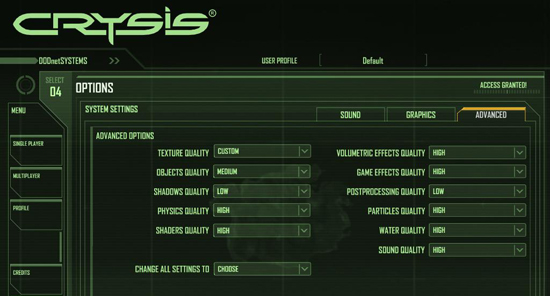
\includegraphics[width=\linewidth]{semana8/crysis_opmenu.jpg} 
\caption{Menu de Opciones del juego \emph{Crysis} presenta configuración de audio y gráficas \cite{crysis}.}
\end{wrapfigure}
Es un menú donde se presenta distintas opciones para modificar el juego, usualmente como mínimo se presentan controles de volumen/audio y dificultad, el menú de opciones suele dividirse en distintas ramas según el tipo de configuración de tal forma se puede tener un menú de opciones para el audio, otro menú de opciones para los controles, otro menú de opciones para la configuración gráfica, menú de opciones para \emph{gameplay} y así muchos mas dependiendo del diseño, alcance y plataforma del vídeo juego. Suele presentarse a través del \emph{Menú de Inicio} pero en algunos juego también puede accederse directamente desde el \emph{gameplay} a través de algún menú de pausa o salida \cite{gb_optionsmenu}.
\subsection{Menú de Partidas (\emph{Save Games})}
Un menú donde se presentan las distintas sesiones de juego guardadas usualmente se presenta información como tiempo de juego, lugar de juego entre otros. Suele presentarse a través del \emph{Menú de Inicio} pero en algunos juego también puede accederse directamente desde el \emph{gameplay} a través de algún menú de pausa o salida.

\begin{wrapfigure}[10]{r}{0.5\linewidth}
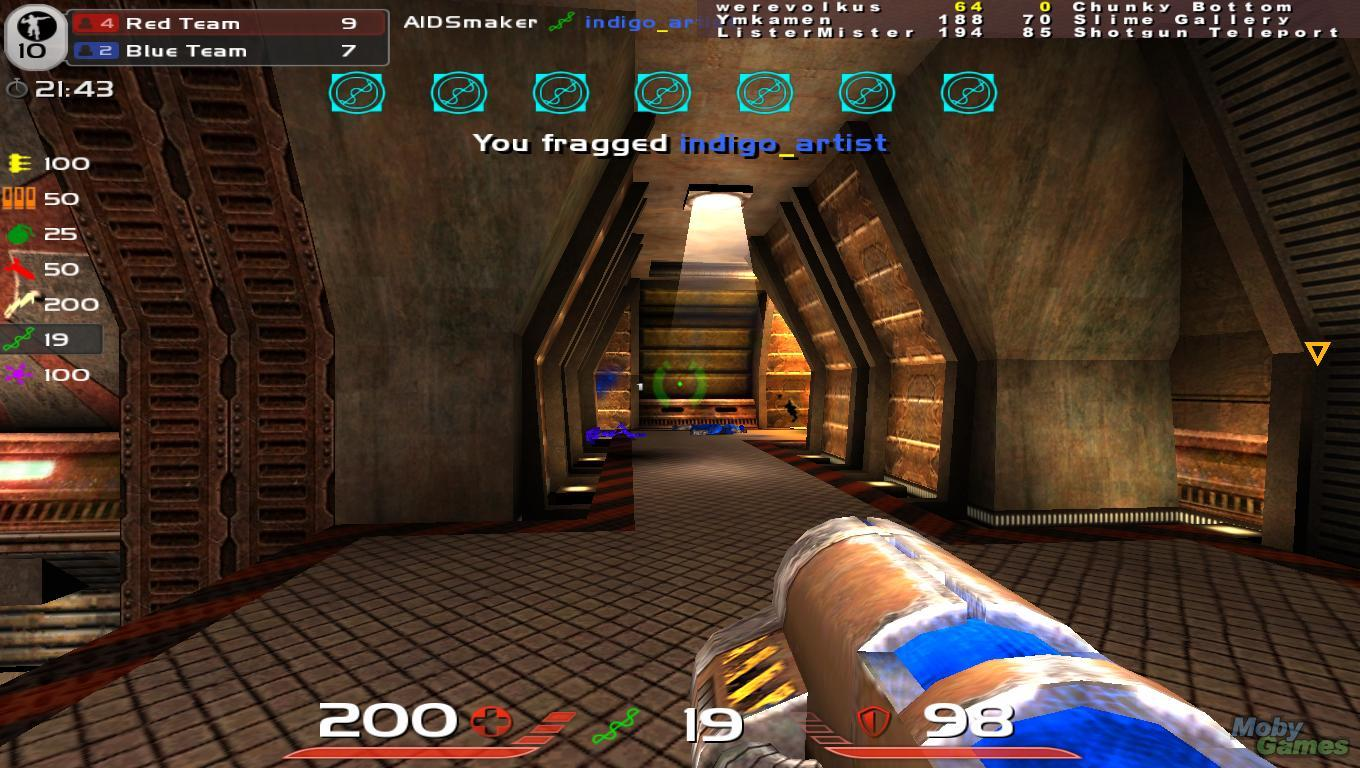
\includegraphics[width=\linewidth]{semana8/quake_live.jpg} 
\caption{HUD del juego \emph{Quake Live} vida, munición y defensa en el panel inferior, armas disponibles en el panel izquierdo y mas \cite{quake_live}.}
\end{wrapfigure}
\subsection{HUD (\emph{Heads-Up Display})}
Interfaz que muestra información del juego en todo momento durante el juego, generalmente se presenta la información de forma concisa y corta utilizando iconos, barras y números. El HUD muestra distinta información, diseño y integración el juego según el tipo de juego y su diseño, usualmente se muestran cosas como numero de vida o cantidad, puntuación, mini-mapa o radar, munición, etc todo esto dependiendo del vídeo juego \cite{huds}.

\section{Actividad}
\todo[inline]{Por hacer.}